\section{Riconoscimento di nuovi architectural smell con Arcan}

%Introduzione
Obiettivo di questo capitolo è l'introduzione e approfondimento dei tre nuovi \textit{architectural smell (AS)} introdotti. Le sezioni successive sono orientate alla descrizione dei tre nuovi \textit{smell}, rappresentati secondo una struttura ben definita:
\begin{enumerate}
    \item Introduzione con descrizione delle cause più comuni che portano al suo inserimento nel sistema e piccola descrizione del nodo introdotto nel grafo
    \item Impatto sulla qualità del codice e possibili strategie di \textit{refactoring}
    \item Strategie di identificazione ideate
    \item Algoritmo di \textit{detection} in pseudocodice
\end{enumerate}
Per favorire la comprensione degli \textit{smell} è necessaria l'introduzione del concetto di \textit{abstraction}, riferito a classi (concrete o astratte) e interfacce che fanno parte del progetto. Questo termine deriva dal \textit{Abstraction Principle} \cite{booch2008object}, che sostiene la semplificazione delle entità attraverso l'eliminazione di dettagli non necessari e la generalizzazione delle caratteristiche condivise tra esse. Un altro principio importante per la comprensione del lavoro svolto è il \textit{Hierarchy Principle} \cite{booch2008object}, che supporta la creazione di un'organizzazione gerarchica di \textit{abstraction} attraverso l'utilizzo di tecniche come classificazione, generalizzazione e sostituibilità.

Obiettivo dell'estensione di Arcan è stato fornire al \textit{tool} la capacità di riconoscere tre nuovi \textit{architectural smells}: \textit{Subclasses Do Not Redefine Methods}, \textit{Unutilizied Abstraction}, e \textit{Unnecessary Abstraction}. 
%In dettaglio, i nuovi smell introdotti sono:
Tutti gli \textit{smell} introdotti violano i principi presentati in precedenza. In dettaglio, lo smell \textit{Subclasses Do Not Redefine Methods} è responsabile della violazione del \textit{Hierarchy Principle} mentre \textit{Unutilizied Abstraction} e \textit{Unnecessary Abstraction} non rispettano il \textit{Abstraction Principle}.


%\input{Tesi/Sezione3-RiconoscimentoSmell/subfiles/3.1_Arcan_e_modifiche}

\subsection{Subclasses Do Not Redefine Methods}
    \textit{Subclasses Do Not Redefine Methods} (\textit{SR}), definito da M. Lippert et al. \cite{lippert2006refactoring}, afferma che se le sottoclassi non ridefiniscono i metodi delle loro superclassi può essere indice del fatto che attraverso l'ereditarietà non è espressa nessuna astrazione ma è più che altro ereditarietà implementativa \cite{lippert2006refactoring}.
        %è uno \textit{smell} definito da M. Lippert e S. Roock \cite{lippert2006refactoring} \cite{SURYANARAYANA201521} che si verifica quando una sottoclasse non ridefinisce nessun metodo della sua superclasse. 
        
    Questo può essere indice del fatto che attraverso la gerarchia non è espressa nessuna astrazione e che non c'è quindi alcun motivo per cui questa gerarchia debba essere presente nel design. 
    La presenza di questo \textit{smell} può essere causata principalmente dalla tendenza all'utilizzo delle gerarchie per il riutilizzo delle funzionalità del padre, senza però che la classe e il suo supertipo condividano una relazione IS-A. 
    
    \paragraph{Nodo di tipo smell nel grafo}
    Il nodo dello \textit{smell} SR dispone di due o più archi in uscita verso altrettante \textit{unit}: 
    \begin{itemize}
        \item Presenta la dipendenza \textit{affects} verso la \textit{unit} colpita dallo \textit{smell}.
        
        \item È in relazione con almeno una \textit{unit} attraverso un arco di tipo \textit{fatherInvolved}, che indica i supertipi della classe che presenta lo \textit{smell}.
    \end{itemize}
    
    %Problemi e refactoring
    \subsubsection{Impatto sulla qualità del codice e refactoring}
        %La presenza di questo smell può influenzare diversi aspetti riguardanti la qualità del codice \cite{SURYANARAYANA201521}, come  comprensibilità, riusabilità, facilità nella modifica ed estensione, affidabilità sono tutti affetti negativamente dalla presenza di \textit{Subclasses Do Not Redefine Methods}. 
        La presenza di \textit{Subclasses Do Not Redefine Methods} può influenzare in maniera negativa la qualità del codice attraverso la compromissione di proprietà quali comprensibilità, riusabilità, facilità nella modifica, estensione e affidabilità \cite{SURYANARAYANA201521}.
        
        Analizzando nel dettaglio le qualità influenzate negativamente dalla presenza di questo \textit{smell}, si può affermare che:
        \begin{itemize}
            \item Quando le classi in una relazione gerarchica non condividono una relazione concettuale IS-A, può portare a molta confusione e ridurre la \textit{comprensibilità} del sistema, confondendo gli sviluppatori e i progettisti.
            
            \item Se le \textit{unit} non condividono una relazione IS-A il riutilizzo del codice potrebbe essere compromesso poiché non è possibile la sostituzione delle istanze dei sottotipi con i loro supertipi. Questa situazione renderebbe difficile il \textit{riutilizzo} dell'intera gerarchia in un altro contesto. Questo potrebbe causare diversi problemi ulteriori relativi alla difficoltà nella \textit{modifica ed estensione} della gerarchia, poiché un cambiamento potrebbe avere un grosso impatto sul codice.
            
            \item La presenza di classi che non condividono una relazione IS-A potrebbe portare a diversi problemi di \textit{affidabilità} del codice, poiché lo scambio tra un'istanza di una superclasse con quella di una sottoclasse potrebbe causare errori indesiderati.
        \end{itemize}
        
        Per il \textit{refactoring} di questo \textit{smell} l'applicazione di \textit{Replace Inheritance With Delegation} è la scelta consigliata e più diffusa \cite{SURYANARAYANA201521}. Questa strategia consiste nella trasformazione della relazione IS-A tra le due classi in una relazione di utilizzo, in modo che la ex-sottoclasse abbia al suo interno un oggetto dell'altra per l'utilizzo dei suoi metodi.
        
        % Considerazioni sullo smell (esempio cosa dell'overloading - già approfondita sopra - , )
    
    %Strategie di identificazione
    \subsubsection{Strategia di identificazione}
        Devo controllare che in ogni relazione gerarchica presente nel programma analizzato non si verifichi la ridefinizione di almeno un metodo del supertipo da parte del sottotipo. Per fare questo, è necessario controllare che l'intersezione dei metodi definiti dalle due classi sia vuota e quindi non abbiano almeno un metodo in comune. 
        Nella ricerca dei metodi definiti dalla superclasse viene utilizzata la funzione \textit{getAllMethods} definita in precedenza poiché, se i metodi delle interfacce non fossero considerati, una situazione analoga a quella definita dalla figura 2, dove il sottotipo (nodo beige) ridefinisce un metodo (nodo verde) definito solamente dall'interfaccia (nodo azzurro) ma non implementato dalla classe astratta (nodo rosso), verrebbe considerata come \textit{smell}. È stato deciso però di non ritenere questa situazione come tale poiché le due classi condividono una relazione IS-A e il metodo dell'interfaccia che la classe concreta implementa è derivato comunque dal suo supertipo.
        %i metodi che la classe astratta può anche non implementare sono stati considerati come fossero \textit{abstract}, ridefiniti poi dalle classi concrete che la estendono.
        \defaultvspace
        \begin{figure}[h]
            \centering
            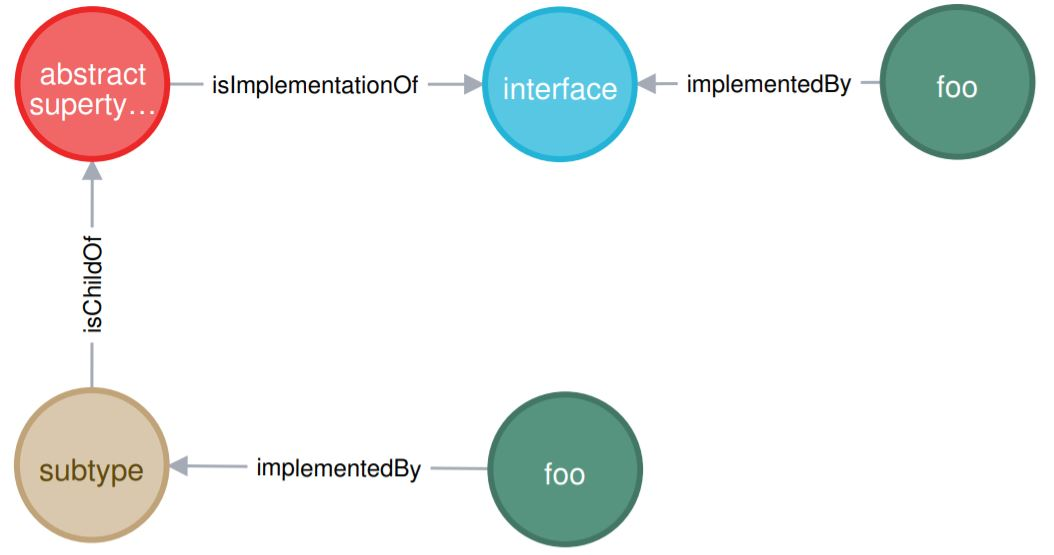
\includegraphics[scale=0.5]{Tesi/Sezione3-RiconoscimentoSmell/immagini/grafo1.JPG}
            \caption{Esempio interfaccia implementata da una classe astratta}
            \label{fig:my_label}
        \end{figure}
        \defaultvspace \\
        %Dalle relazioni considerate vengono escluse però quelle gerarchiche tra due interfacce, p
        %Per l'identificazione di questo smell inoltre non sono state considerate due diverse categorie di unit:
        Dalle relazione \textit{isChildOf} considerate vengono escluse tutte quelle che coinvolgono:
        \begin{itemize}
            \item Due \textit{unit} \textit{interface}, poichè nelle gerarchie tra interfacce non avviene la ridefinizione di metodi ma si verifica solamente l'estensione del comportamento attraverso nuove funzioni, pertanto tutti questi casi risulterebbero falsi positivi.
            
            \item Una \textit{unit} di tipo classe che rappresenta una \textit{exception} (oppure anche \textit{error}), poiché è molto comune che abbiano come supertipo una \textit{exception} e richiamino solamente il costruttore utilizzando parametri diversi. In questi casi non c'è ridefinizione dei metodi ma non è stato giudicato comunque come \textit{smell}, in quanto la relazione IS-A è presente.
        \end{itemize}
        %
        % tutte le coppie di nodi di tipo classe che condividono una relazione \textit{isChildOf} dove
        In termini di grafo è necessario considerare tutti i nodi che presentano un arco \textit{isChildOf} in uscita dove almeno un nodo di tipo \textit{function} in ingresso al nodo considerato non condivida la proprietà \textit{name} con un'altro nodo \textit{function}:
        \begin{itemize}
            \item Definito da uno dei supertipi della classe analizzata, dove per supertipi si intendono i nodi che hanno in ingresso gli archi \textit{isChildOf} provenienti dalla classe sotto analisi.
            
            \item Presente nella gerarchia di uno dei supertipi. Per verificare questo si seguono tutti gli archi \textit{isChildOf} e \textit{implementedBy} a partire dai supertipi al fine di controllare anche tutti i metodi ereditati.
        \end{itemize}
        %In termini di grafo bisogna considerare tutte le coppie di nodi di tipo classe che condividono una relazione isChildOf dove il nodo del supertipo non ha in ingresso un nodo function che condivide il nome con almeno un nodo function che la unit padre ha in ingresso. 
        %Inoltre è necessario risalire la gerarchia seguendo le relazioni \textit{isChildOf} per verificare che il sottotipo non abbia un nodo function 
        %Inoltre è necessario anche risalire la gerarchia della classe padre per verificare che il sottotipo non ridefinisca qualche metodo che il padre erediti dalla sua gerarchia, poichè il parser delle funzioni non include nella unit eventuali metodi ereditati. DA MIGLIORARE LE InFo sUL GRAFO
        
    
    %Algoritmo
    \subsubsection{Algoritmo}
        \paragraph{Input} un sottografo del grafo principale, considerando solamente i nodi che rappresentano classi (concrete e astratte) coinvolte in una dipendenza del tipo \textit{isChildOf} e le relative funzioni definite dalle classi. Oltre all'arco \textit{isChildOf} sarà considerato anche \textit{implementedBy}.
        %Gli archi considerati sono invece di tipo \textit{isChildOf} e \textit{implementedBy}
    
        \paragraph{Output} una lista di classi che presentano lo \textit{smell} e i relativi supertipi coinvolti.
        
        \paragraph{Algoritmo}
            \begin{algorithmic}
    \Function{Subclasses-does-not-redefine-methods-detector}{ }
        \State{Prendo tutti i nodi che hanno almeno un arco in entrata del tipo}
        \State{isChildOf, escludendo le interfacce e le enumerazioni}
        \For{Ogni vertice trovato, che rappresenta il supertipo}
            \State{Prendo la lista delle funzioni definite ed ereditate dalla unit,}
            \State{includendo anche quelli definiti dalle interfacce implementate}
            \If{La lista dei metodi considerata non è vuota}
                \For{Ogni sottotipo con isChildOf in uscita verso il supertipo}
                    \State{Prendo la lista di tutte le funzioni definite dal sottotipo}
                    \If{L'intersezione tra le liste dei metodi è l'insieme vuoto}
                        \State{Aggiungo il vertice alla lista degli smell}
                    \EndIf
                \EndFor
             \EndIf
        \EndFor
    \EndFunction
\end{algorithmic}
    


\subsection{Unutilizied Abstraction}
    \textit{Unutilizied Abstraction} (\textit{UUA}), definito da G. Suryanarayana et al. \cite{SURYANARAYANA201521}, si manifesta quando una \textit{abstraction} viene lasciata inutilizzata, cioè non direttamente usata o non raggiungibile. Questo \textit{smell} si può manifestare in due forme: 
        \begin{itemize}
        \item \textit{Unreferenced Abstraction}, classi concrete che non sono utilizzate da nessuno.
        
        \item \textit{Orphan Abstraction}, classi astratte e interfacce che non hanno nessuna abstraction derivata.
    \end{itemize}
    %
    Il principio di astrazione afferma che le \textit{abstraction} dovrebbero avere loro assegnate responsabilità singole e limitate. La presenza di classi e interfacce senza uno scopo specifico nel design e quindi inutilizzate viola il principio, introducendo nel design questo \textit{smell}. Un altro principio violato oltre a quello di astrazione è il principio \textit{YAGNI (You Aren't Gonna Need It} \cite{yagniFowler}, che raccomanda di evitare l'aggiunta di funzionalità non strettamente necessarie al design.

    Le cause che possono portare all'introduzione di \textit{UNA} nel design sono:
    \begin{itemize} %Sicuramente sistemare la forma - 
        \item \textit{Design speculativo}: l'introduzione nel design di funzionalità e strutture che potrebbero servire in futuro può portare alla violazione del principio \textit{YAGNI} \cite{yagniFowler} e all'introduzione di \textit{abstraction} attualmente non utilizzate.
            %una condizione che si verifica quando i progettisti introducono nel design funzionalità e strutture che potrebbero servire in futuro, violando il principio You Aren't Gonna Need It \cite{yagniFowler}.
            % la tendenza allo sviluppo orientata al futuro è una condizione che si verifica quando
        
        \item \textit{Cambio di Requisiti}: il cambiamento di requisiti del progetto potrebbe avere influenza anche sulle \textit{abstraction} impiegate, perciò alcune potrebbero rimanere orfane e non utilizzate.
            %non è anomalo che durante lo sviluppo di un nuovo sistema i requisiti dello stesso cambino in continuazione, portando agli sviluppatori una continua attività di modifiche e cambi al progetto; proprio per questo motivo, sono stati introdotti i metodi agili \cite{checosa?}. Questi continui cambi di requisiti hanno effetto sulle funzionalità e soprattutto sulle abstraction utilizzate del progetto, che potrebbero quindi non essere più utilizzate e rimanere orfane nel design.
        
        \item \textit{Cancellazione parziale delle abstraction}: quando la \textit{manutenzione} di un progetto viene effettuata senza cancellare \textit{abstraction} vecchie e non più utili per il design, lasciando così nel sistema diverse \textit{unutilizied abstraction}.
            % durante la manutenzione di un progetto, si effettuano diverse attività tra cui appunto la cancellazione delle abstraction non più attive. Se quest'ultima attività viene effettuata parzialmente o non viene proprio svolta, potrebbero rimanere nel progetto abstraction vecchie e che non servono più al design, lasciando così nel sistema diverse Unutilized Abstraction.
        
        \item \textit{Paura di rompere il codice}: la cancellazione di \textit{abstraction} potrebbe portare diversi problemi ai programmatori poiché spesso essi decidono di non rimuoverle per paura che vengano ancora utilizzate nel codice. L'introduzione dello \textit{smell} causata da questo timore si verifica soprattutto in progetti che presentano un grande numero di classi e linee di codice.
        %quando non viene effettuata la cancellazione di abstraction poichè i programmatori hanno paura che quella classe sia ancora utilizzata da qualche parte nel codice e che quindi la loro cancellazione possa portare svariati problemi. Questa condizione si verifica soprattutto in grandi progetti con molte classi e loc.
    \end{itemize}
    
    \paragraph{Nodo di tipo smell nel grafo}
        Il nodo dello \textit{smell} UUA si presenta come un nodo di tipo \textit{smell} con una singola dipendenza verso la classe che presenta il problema.
    
    
    %Impatto
     \subsubsection{Impatto sulla qualità del codice e refactoring}
         \textit{Unutilizied Abstraction} ha un impatto fortemente negativo su due qualità del progetto, ovvero affidabilità e facilità di comprensione del sistema. La presenza di molte classi inutilizzate infatti potrebbe portare ad errori a run-time, se per esempio una di queste dovesse venire erroneamente invocata portandosi dietro piccoli \textit{bug}. Inoltre l'inquinamento del design da parte di molte classi e interfacce diminuisce la comprensione del progetto aumentandone il carico cognitivo, causando anche problemi secondari come difficoltà nello studio del funzionamento del sistema oppure estensione e manutenzione del codice complicate.
         %e può portare a diversi problemi secondari come difficoltà a studiare il funzionamento del prodotto oppure problemi con l'estensione o la manutenzione del codice.
        
        La tecnica di \textit{refactoring} consigliata è l'eliminazione del progetto di tutte le \textit{abstraction} non più necessarie. Nel caso di API pubbliche però l'eliminazione potrebbe non essere la soluzione opportuna, poiché alcune di esse potrebbero ancora essere utilizzate da qualche \textit{client}. La soluzione in questo caso è la segnalazione delle \textit{unutilizied abstraction} come deprecate.
        % Nel caso di API pubbliche che possono essere ancora utilizzate da qualche client invece, è opportuno segnalare come deprecate le abstraction coinvolte.

    %Problemi
    
    %Considerazioni fatte sullo smell (Esempio la cosa dell'overloading per SR)
    
    %Strategie di identificazione
    \subsubsection{Strategie di identificazione}
        Per l'identificazione dello \textit{smell} \textit{Unutilizied Abstraction} è necessaria l'identificazione di tutte le \textit{abstraction} del progetto inutilizzate oppure non utilizzate per il loro naturale scopo. In particolare, come già analizzato nella sua introduzione, bisogna considerare tutte quelle che appartengono a due differenti categorie:
        \begin{itemize}
            \item \textit{Unreferenced Abstractions}, classi concrete non utilizzate da nessuno e senza alcun riferimento all'interno del progetto, interpretato nel grafo come i nodi che non presentano in ingresso alcun arco \textit{dependsOn} proveniente da una classe esterna.
            Quest'ultima precisazione viene specificata poiché nel grafo di Arcan le \textit{inner class} hanno sempre una relazione \textit{dependsOn} verso il loro contenitore e, senza questa specificazione, le classi \textit{unreferenced} contenenti almeno una classe interna non utilizzata non sarebbero state erroneamente considerate come \textit{smell}. 
            L'utilizzo di una classe interna da parte di una esterna genera invece nel grafo due differenti archi \textit{dependsOn}, uno in ingresso alla classe utilizzata e l'altro a quella che la contiene. In questo caso, anche se la classe contenitore non viene utilizzata, non viene giustamente considerato come \textit{smell}.  
            
            \item \textit{Orphan Abstractions}, classi astratte o interfacce che non vengono implementate o estese. Per quanto riguarda le classi astratte, bisogna ricercare nel grafo tutti i nodi che le rappresentano senza nessun arco \textit{isChildOf} in ingresso; i nodi di tipo interfaccia invece non devono presentare in ingresso, oltre ad archi \textit{isChildOf}, nemmeno nessuna relazione di tipo \textit{isImplementationOf}.
            %, ovvero nodi del grafo di tipo classe astratta e interfaccia che non presentano nessun arco di tipo \textit{isChildOf} in ingresso, oppure nodi interfaccia che non presentano archi \textit{isImplementationOf} in ingresso. 
            In questo caso non si deve porre molta attenzione alle classi interne, poiché per la \textit{detection} di questo caso non vengono presi in considerazione gli archi del tipo dependsOn.
        \end{itemize}
        
    \subsubsection{Algoritmo}
        \paragraph{Input} un sottografo del grafo principale considerando solamente i nodi che rappresentano classi e interfacce e gli archi \textit{isChildOf}, \textit{dependsOn} oppure \textit{isImplementationOf}. 
        
        \paragraph{Output} una lista di unit che presentano lo \textit{smell}.
        
        \paragraph{Algoritmo}
        \begin{algorithmic}
\Function{unutilizied-abstraction-detector}{}
\State{Prendo la lista di tutti i nodi unit}
\For{Ogni vertice della lista}
    \If{Il vertice è di tipo classe o enum}
        \State{Considero tutti i nodi con un arco dependsOn in uscita verso}
        \State{il vertice}
    \EndIf
    \If{Il vertice è di tipo classe astratta}
        \State{Considero tutti i nodi con un arco isChildOf verso il vertice}
    \EndIf
    \If{Il vertice è di tipo interfaccia}
        \State{Considero tutti i nodi con un arco dependsOn oppure }
        \State{isChildOf verso il vertice}
    \EndIf
    
    \If{I nodi considerati sono 0 oppure sono tutti classi interne}
        \State{Aggiungi il nodo alla lista degli smell}
    \EndIf
    
\EndFor
\EndFunction 
\end{algorithmic}


    

\subsection{Unnecessary Abstraction}
    \textit{Unnecessary Abstraction} (\textit{UNA}), definito da G. Suryanarayana et al. \cite{SURYANARAYANA201521}, si verifica quando un \textit{abstraction} che non è in realtà necessaria (e quindi potrebbe essere evitata) viene introdotta nel design.
    Questo \textit{smell} viola il principio di astrazione, poiché si verifica l'introduzione nel design di \textit{abstraction} con responsabilità limitate oppure nulle.
    
    Si possono riassumere tre cause principali che portano l'introduzione di questo \textit{smell} nel design:
        %Le cause principali dell'introduzione di questo \textit{smell} nel sistema si possono riassumere in tre differenti casi:
    \begin{itemize}
        \item \textit{Utilizzo improprio di feature del linguaggio:}
        \textit{abstraction} non necessarie possono essere introdotte nel design solamente per convenienza, utilizzando \textit{feature} del linguaggio in maniera impropria. Il caso più diffuso è rappresentato dalle \textit{constant placeholder}, interfacce o classi utilizzate dal programmatore solamente per contenere valori costanti.
        La generazione di queste \textit{abstraction} consente al programmatore di implementare o estendere il \textit{placeholder} nella classe desiderata in modo da utilizzare una costante senza la necessità di specificarne il tipo ma solamente attraverso il suo nome.
        
        \item \textit{Over-engineering:} vengono definite \textit{over engineered} le \textit{abstraction} introdotte nel design che risultano superflue e prive di un grande significato associato. 
        Un esempio di classe over engineered è mostrato dalla figura 3, dove sono presenti una classe \textit{Customer} contenente un attributo ID che, invece di essere di tipo \textit{String}, è incapsulato da una classe \textit{CustomerID} dedicata, superflua e non necessaria per il sistema.
        %Un esempio di questo caso può essere rappresentato da una classe Customer contenente un attributo CustomerID che, al posto di essere un attributo \textit{String} di Customer, ha una classe CustomerID dedicata che presenta getter e setter, costruttore e appunto un parametro ID di tipo \textit{String}. CustomerID risulta quindi superflua e non necessaria per il sistema.
        \begin{figure}[h]
            \centering
            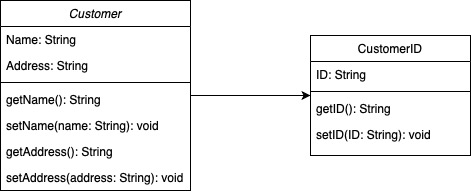
\includegraphics[scale=0.45]{Tesi/Sezione3-RiconoscimentoSmell/immagini/Untitled Diagram.jpg}
            \caption{Esempio di classe over engineered}
            \label{fig:my_label}
        \end{figure}
        
        
        \item \textit{Procedural thinking:} %si verifica quando lo sviluppatore, soprattutto se sè è affacciato di recente allo sviluppo object-oriented, tende a pensare le classi in modo procedurale.
        se uno sviluppatore, spesso affacciato recentemente allo sviluppo Object Oriented, tende a pensare le classi in maniera procedurale e non dotate di responsabilità e compiti, può introdurre nel codice \textit{abstraction} non necessarie. 
        Questa tendenza si traduce in classi che "svolgono procedure" invece di "essere qualcosa" violando il principio di astrazione, a causa di responsabilità multiple e poco definite. Un esempio di classe procedurale possono essere le classi di \textit{utilities}.
    \end{itemize}
    
    
    \paragraph{Nodo di tipo smell nel grafo}
        Il nodo dello \textit{smell} presenta un'unica dipendenza verso la sospetta \textit{Unnecessary Abstraction}. Inoltre ha una proprietà chiamata \textit{unnecessaryCase}, che indica quale delle tre casistiche di \textit{UNA} è stata riscontrata nella \textit{unit}.
        
            
    %Problemi e refactoring
    \subsubsection{Impatto sulla qualità del codice e refactoring}
        \textit{Unnecessary Abstraction} ha un impatto significativo sulla possibilità di riutilizzo del codice e sulla comprensione del progetto. 
        Riguardo la comprensione, la presenza di numerose interfacce non necessarie incide in maniera negativa poiché aumenta la complessità del design, causando una maggiore difficoltà nell'interpretazione del design e nella chiarezza del progetto.
        
        Anche il riutilizzo del codice subisce un influenza negativa dalla presenza di \textit{Unnecessary Abstraction} poiché \textit{abstraction} senza responsabilità uniche e ben definite e specializzate per un design particolare risultano molto difficili da riutilizzare in contesti differenti.
        
        Se inoltre viene utilizzata un'interfaccia come \textit{constant placeholder} possono verificarsi ulteriori problemi:
        \begin{itemize}
            \item Le classi derivate da quelle che implementano l'interfaccia possono risultare inquinate da costanti che non sono rilevanti per loro.
            
            \item Si verifica una violazione dell'incapsulamento in quanto vengono mostrati, attraverso l'interfaccia, dettagli implementativi.
            
            \item Quando le costanti sono presenti nelle interfacce, cambiamenti ad esse possono creare problemi ai \textit{client} esistenti.
            
            \item Le interfacce rappresentano un protocollo che le classi che lo implementano devono rispettare e l'utilizzo come \textit{constant placeholder} è un abuso del meccanismo di astrazione.
        \end{itemize}
        
        Al fine di rimuovere questo problema dal codice ed aumentare la qualità dello stesso, sono suggerite tre diverse strategie \cite{SURYANARAYANA201521} di \textit{refactoring}:
        \begin{itemize}
            \item Le classi procedurali dovrebbero essere eliminate, secondo quanto proposto da Fowler \cite{fowler2018refactoring}.
            
            \item Si suggerisce l'eliminazione delle \textit{constant placeholder} per favorire l'utilizzo di costrutti forniti dal linguaggio che si adattano meglio a questa esigenza (un esempio possono essere le enumerazioni).
            
            \item Per le classi \textit{over engineered} Fowler consiglia \cite{fowler2018refactoring} l'applicazione del \textit{Inline Class Refactoring}, che consiste nell'unione delle due classi in una sola. Riferendoci all'esempio presentato in precedenza, l'azione suggerita è l'aggiunta di un parametro \textit{CustomerID} di tipo \textit{String} alla classe \textit{Customer}, eliminando la classe \textit{CustomerID} non necessaria.
        \end{itemize}
        
    
    %Considerazioni fatte sullo smell (Esempio la cosa dell'overloading)
    
    %Strategie di identificazione
    \subsubsection{Strategia di identificazione}
        Le regole di identificazione di \textit{Unnecessary Abstraction} sono state divise in tre differenti casistiche, in base alle cause della presenza di questo \textit{smell} definite nella sezione 4.3. Vengono considerate per la valutazione della presenza di \textit{UNA}:
        \begin{itemize}
            \item \textit{Placeholder abstraction} classi oppure interfacce senza alcuna funzione definita al loro interno che contengono solamente attributi costanti. La ricerca di queste classi ha visto l'esclusione di due categorie principali di \textit{unit}, in quanto risultanti come falsi positivi. Non sono state considerate le enumerazioni, poiché sono per definizione contenitori di costanti, e tutte le classi \textit{exception} o \textit{error}, poiché anche se presentano le caratteristiche delle \textit{constant placeholder} non possono essere considerate come tali. Sono state escluse inoltre tutte le classi che presentano un supertipo, con le uniche eccezioni di  padri vuoti oppure contenenti solamente costanti.
            
            Nel grafo le \textit{placeholder abstraction} vengono rappresentate da tutti i nodi senza archi in ingresso di tipo \textit{implementedBy} e, per ogni arco in ingresso del tipo \textit{definedBy}, il nodo corrispondente all'attributo deve avere i parametri \textit{constantAttribute} e \textit{defaultValue} aventi il valore \textit{true}.
            Vengono esclusi dalla ricerca tutti i nodi \textit{unit} che presentano \textit{componentType} con valore \textit{enum} oppure con nomi che terminano con le stringhe \textit{"Error"} oppure \textit{"Exception"}. Inoltre per le \textit{unit} che presentano  archi \textit{isChildOf} in uscita viene controllato che i supertipi non presentino alcun arco in ingresso oppure che presentino le stesse caratteristiche definite in precedenza.
        
            
            \item \textit{Over-engineered} classi concrete che definiscono solamente un attributo e due funzioni, rappresentanti i metodi \textit{getter} e \textit{setter}. Inoltre queste classi devono essere definite come attributo in solamente un'altra \textit{abstraction} e non possono presentare alcun supertipo che non sia vuoto, poiché altrimenti la classe subirebbe una modifica a causa degli elementi ereditati. Per la definizione di queste regole si è replicato il caso descritto dalla figura 3. È stato deciso inoltre di inserire il limite di solamente un utilizzo come parametro da un'altra \textit{abstraction} poiché altrimenti la classe potrebbe avere significato nel sistema di riferimento, come avviene ad esempio nell'applicazione del pattern \textit{Object Identifier} \cite{brown1996pattern}. 
            
            Le condizioni per l'identificazione si traducono nella ricerca di nodi del grafo che presentano in ingresso un solo arco di tipo \textit{definedBy} e massimo due \textit{implementedBy}. Viene controllato anche che il nome di ogni funzione rappresentata dall'arco \textit{implementedBy} sia effettivamente una funzione \textit{getter} o \textit{setter} per l'attributo della classe, ovvero presenti un nome del tipo \{get/set\}\{nomeAttributo\}. Inoltre il nodo deve presentare solamente un arco in ingresso di tipo dependsOn da un'altra \textit{unit}, che a sua volta ha in ingresso un'arco \textit{containedIn} da un attributo dello stesso tipo della classe sotto esame.
            Se infine il nodo presentasse un arco in uscita di tipo \textit{isChildOf}, la \textit{unit} del supertipo non dovrebbe aver alcun arco in ingresso \textit{definedBy} oppure \textit{implementedBy} ed anche eventuali supertipi di questa \textit{unit} non dovrebbero presentare nessun arco di queste due tipologie. Un esempio di questa struttura può essere osservato nella figura 4 (dove alla classe Customer è stato aggiunto un ulteriore attributo \textit{name}).
            % Non considerate classi con il parametro final e default 
            
            \begin{figure}[h]
                \centering
                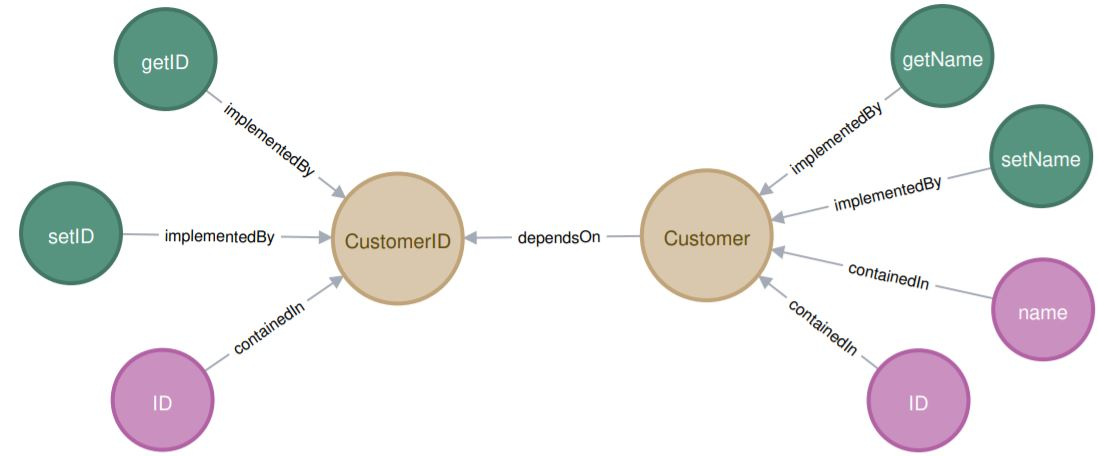
\includegraphics[scale=0.6]{Tesi/Sezione3-RiconoscimentoSmell/immagini/overengineered.JPG}
                \caption{Esempio classi overengineered nel grafo}
                \label{fig:my_label}
            \end{figure}
           
           
           \item \textit{Procedural class} classi concrete o astratte senza attributi e con solamente una oppure due funzioni definite al loro interno. Non sono state considerate nella ricerca tutte quelle classi che presentano dei supertipi, per due motivi principali. In primo luogo, se la classe avesse dei supertipi potrebbe ereditare metodi e attributi che potrebbero far sì che non rispetti più i vincoli appena definiti. Inoltre le classi procedurali sono spesso introdotte da persone non esperte nella programmazione orientata agli oggetti e prive di significato nel design, cosa che potrebbe non verificarsi se è presente una gerarchia.
            
           % Queste strategie si traducono in termini di grafo con tutti 
            Per quanto riguarda il grafo, bisogna ricercare i nodi con \textit{componentType} di valore \textit{class} oppure \textit{abstract\_class} che presentano in ingresso uno oppure due archi di tipo \textit{implementedBy} e nessun arco di tipo \textit{containedIn} in ingresso oppure \textit{isChildOf} in uscita.
        \end{itemize}
        
    %Algoritmo
    \subsubsection{Algoritmo}
        \paragraph{Input} un sottografo del grafo principale, contenente i nodi \textit{unit} e le \textit{function} e \textit{attribute} che esse definiscono. Gli archi considerati sono di tipo \textit{dependsOn}, \textit{implementedBy} e \textit{definedIn}. 
        
        \paragraph{Output} la lista delle classi affette da questo \textit{smell} e la relativa causa che ha portato alla loro identificazione. 
        
        \paragraph{Algoritmo}
            \begin{algorithmic}
    \Function{unnecessary-abstraction-detection}{G}
        \State{Prendo la lista di tutti i vertici di tipo unit}
        \For{Ogni vertice nella lista}
            %Procedural
            \If{\Call{is-procedural-class}{vertice}}
                \State{Aggiungo il vertice alla lista degli smell}
            \EndIf
            %Costant
            \If{\Call{is-constant-placeholder}{vertice}}
                \State{Aggiungo il vertice alla lista degli smell}
            \EndIf
            %Over
            \If{\Call{is-over-engineered}{vertice}}
                \State{Aggiungo il vertice alla lista degli smell}
            \EndIf
        \EndFor
    \EndFunction
    \\
    \Function{is-procedural-class}{vertice}
        \If{Il vertice è una classe concreta o astratta}
            \If{Il vertice non ha archi in ingresso containedIn}
                \If{Il vertice non ha archi in uscita isChildOf}
                    \If{Il vertice ha 1-2 archi in ingresso implementedBy}
                        \State{\textbf{return} la classe è una Unnecessary Abstraction}
                    \EndIf
                \EndIf
            \EndIf
        \EndIf
    \EndFunction
    \\
    \Function{is-constant-placeholder}{vertice}
        \If{Il vertice non rappresenta enumerazioni o classi di errore}
            \If{La classe non ha archi in ingresso implementedBy}
                \If{La classe ha archi in uscita isChildOf}
                    \If{Almeno un supertipo non è una constant placeholder op-\\\hspace{2.3cm}pure non è vuoto}
                        \State{\textbf{return} la classe non è una Unnecessary Abstraction}
                    \EndIf
                \EndIf

                \If{Tutti i nodi con arco containedIn verso questo vertice hanno \\\hspace{1.7cm} gli attributi constantAttribute e defaultValue true}
                    \State{\textbf{return} la classe è una Unnecessary Abstraction}
                \EndIf
            \EndIf
        \EndIf
    \EndFunction
    \\
    \Function{is-over-engineered}{vertice}
        \If{Il vertice ha un solo arco in ingresso containedIn}
            \If{Il vertice ha max 2 archi implementedBy in ingresso con nomi \\\hspace{1.1cm} delle funzioni collegate corrispondono a getNomeAttributo oppure \\\hspace{1.1cm} setNomeAttributo}
                \If{Il vertice ha solo un'arco in ingresso dependsOn da un vertice \\\hspace{1.7cm} che definisce un attributo dello stesso tipo della classe rappresen- \\\hspace{1.7cm}tata dal vertice}
                    \State{\textbf{return} la classe è una Unnecessary Abstraction}
                \EndIf
            \EndIf
        \EndIf
    \EndFunction
\end{algorithmic}

    

